\vspace{-0.2mm}
\section{Results}\label{sec:exp}
In this section, we implement our classifiers to evaluate their performance on user profiles described in part~\ref{simpleuser} writing more than a thousands lines of code in Python. First, for each classifier, we declare the user profile(s) that we use for evaluation of its performance and the false data that we use for computing its false positive. Second, we describe the result of each classifier and give a summary and comparison of them at the end of this section. 

\subsection{User Profiles and False Data}

For each classifier, we use a specific user profile and depending on that we choose the false data. As we explained above, false data is the base traffic that we use to compute false positive. Note that, we use same length of traffic for \bc and the false data. In other words, it is the traffic that we compare our \bc traffic with. For example, when we have 10 minutes of HTTP traffic, we are continuously browsing different websites for 10 minutes. We make these samples by concatenating the browsing of different websites.
 In the following, we describe these pairs for each classifier(s). 
\begin{compactitem}

\item For shape-based classifier, we use the simple user profile. Furthermore, we use HTTP which is the typical user behavior as the false data. This experiment evaluates if \bc traffic can be differentiated from browsing an HTTP website. 
\item  For the rest of the binary classifiers in this section, we use simple noisy user profile and attempt to detect the presence of \bc. Note that, similar to the window-based classifier, we use HTTP for the false data. This experiment attempts to evaluate if browsing an HTTP website is enough to hide the \bc traffic. 
\item For the neural network-based and combined classifiers, we use the complex web and complex CAIDA user for training and testing.
\end{compactitem}
Note that, for these two classifiers, we evaluate our model using $10,000$ number of test data, and report the false positive, true positive and accuracy. For rest of the classifiers, we use $500$ number of test data for evaluation. Also, the data is balanced, which means we have the same number of data for each category.

%\subsection{Shape-based Classifier}
\begin{comment}
 \begin{figure*}[!t]
\begin{subfigure}{.48\linewidth}
\centering
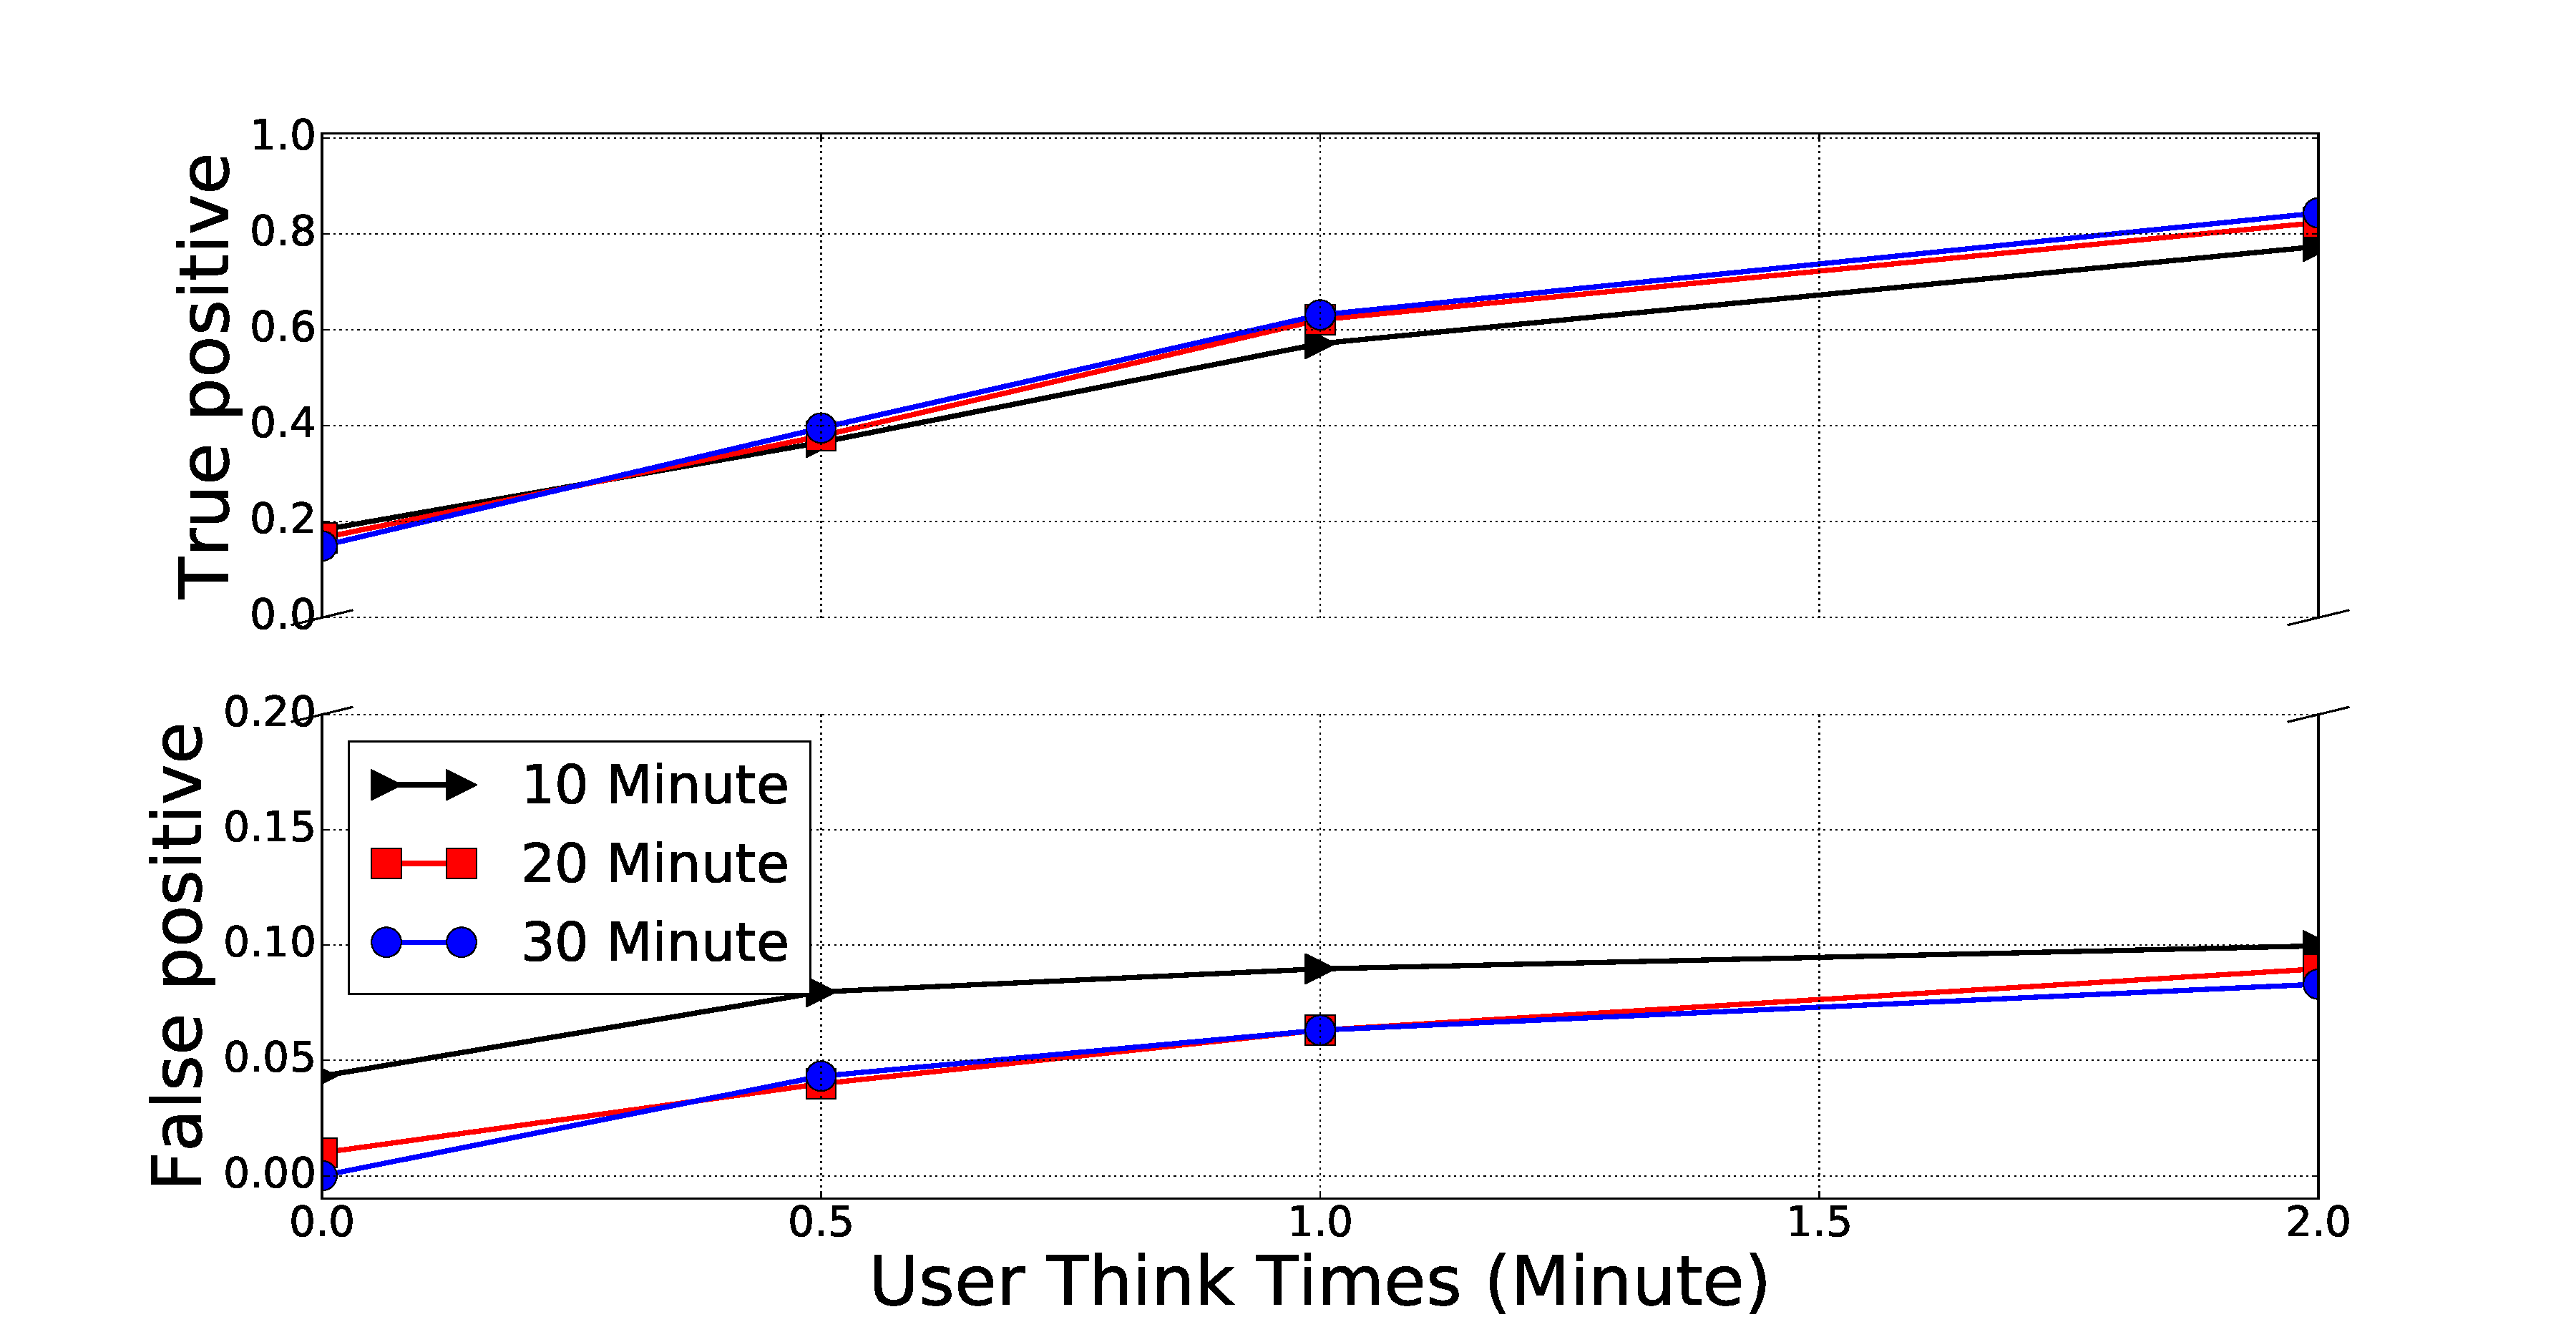
\includegraphics[width=\linewidth]{image/jan25/full_d2u.pdf}
\caption{Full Mode}
\label{fig:tp}
\end{subfigure}
\centering
\begin{subfigure}{.48\linewidth}
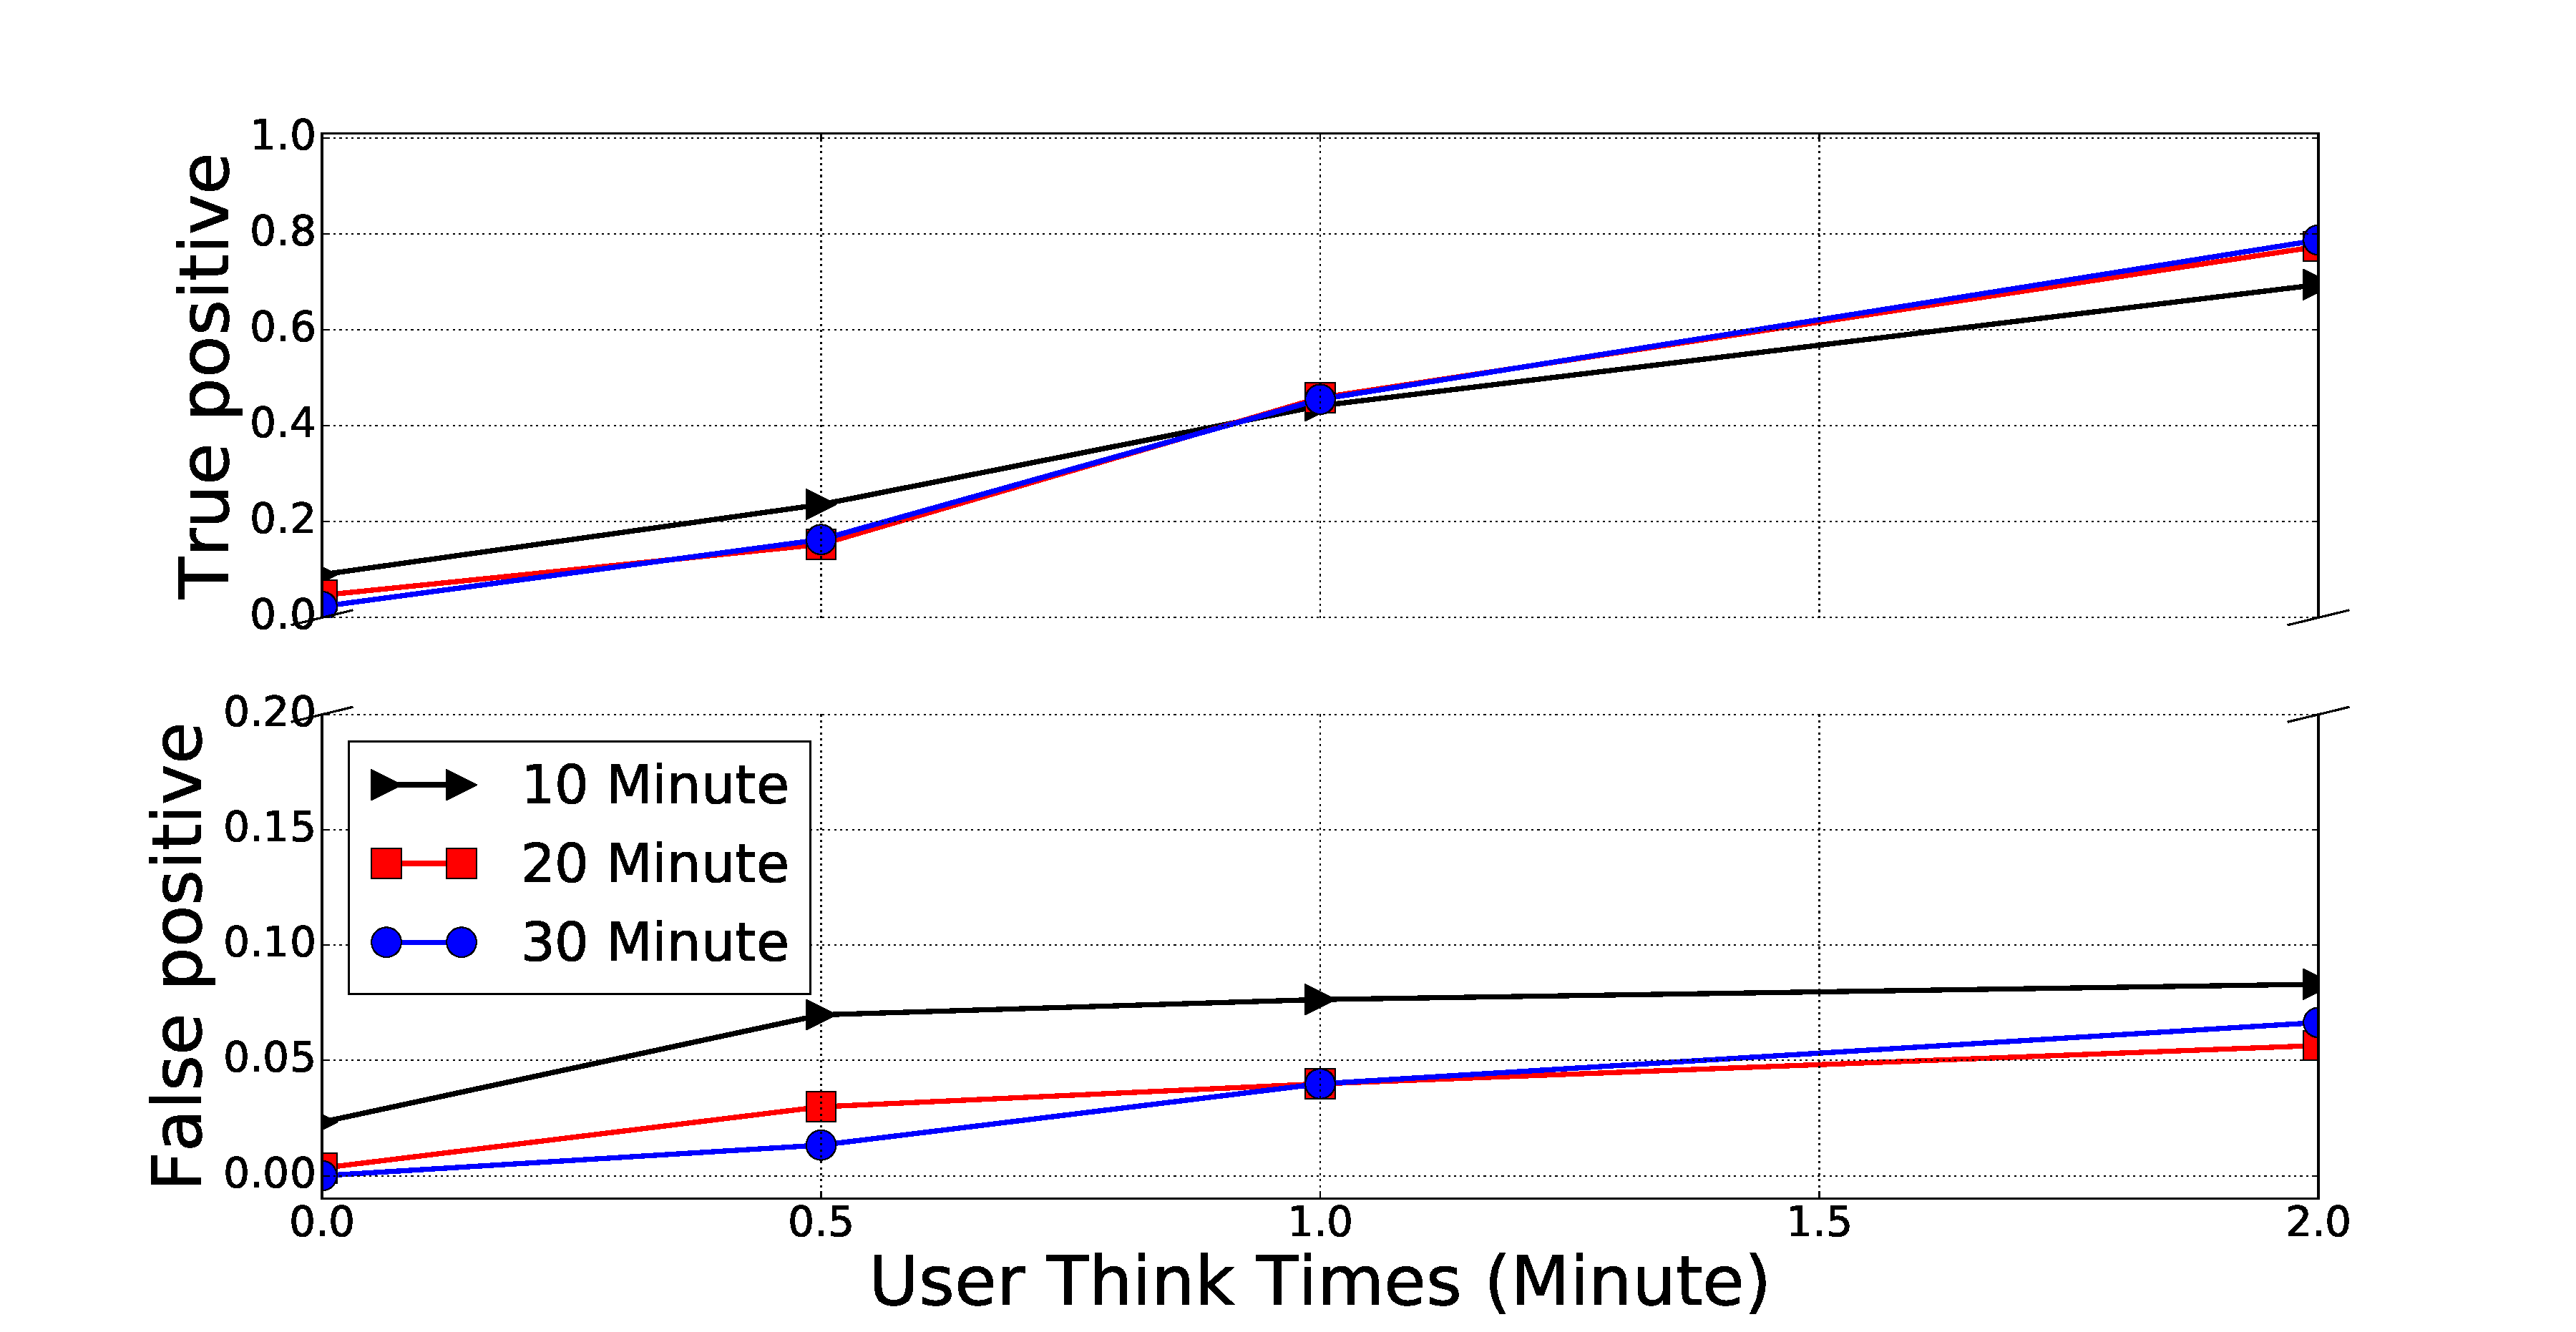
\includegraphics[width=\linewidth]{image/jan25/cmp_d2u.pdf}
\caption{Compact Mode}
\label{fig:fp}
\end{subfigure}
\caption{Result of \code{D2U} classifier on noisy \bc traffic}
\label{fig:d2u}
\end{figure*}
\end{comment}

\subsection{Size-based Classifiers}

\subsubsection{\code{SizeHist} Classifier}
%For this classifier, we compute the histogram of packet sizes and using a correlation algorithm we decide if the traffic contains \bc or not. Because of the \bc specific packet sizes, we expect to have a good performance even in the presence of background noise.
We implement the \code{sizeHist} classifier on \bc traffic in compact and full block modes using the noisy user model described in Section~\ref{simpleuser}. Figure~\ref{fig:sizeHist_non} shows the performance of this classifier. We control the noise using think time (T). Increasing T decreases the noise and enhances the classifier's performance. Figure~\ref{fig:sizeHist_non} shows that we can reach more than $90\%$ true positive and $0\%$ false positive for both modes when we have $10$ minutes of traffic and set T to $2$ minutes. It is worth stating that we could reach similar results when we set T to $0.5$ minutes and have $20$ minutes of traffic.

%impact of traffic length and background noise on true positive and false positive for this classifier. 
 
\begin{comment}
\subsubsection{The \code{D2U} Classifier}
We showed in Appendix~\ref{sec:charachterzing_bc} that downstream to upstream ratio of \bc traffic could be a distinguishing factor to identify \bc from other traffics. D2U classifier attempts to use the symmetry between upstream and downstream of \bc traffic to distinguish it from other protocols. Figure~\ref{fig:d2u} shows the result of this classifier on noisy user profile for full and compact block modes. It indicates that increasing T and thus decreasing the background noise on \bc traffic would improve the 
detection rate. More specifically, our true positive enhances from $0$ to $80\%$ when we increase T from $0$ to $2$ minutes.
\end{comment}


\subsection{Shape-based Classifier}
%As we explained in Section~\ref{window-sec}, shape-based classifier attempts to detect \bc blocks using the volume of traffic downloaded at a time window around the block announcements times, and using the block detection rate it computes the true and false positive.
To implement this classifier, we set $J$ and $\omega$ introduced in Section~\ref{window-sec} to $100$ kilobytes and $20$ seconds, respectively. 
To set $\eta$, we compute block detection rate for \bc using ground false shown in Figure~\ref{fig:window}. We need to set $\eta$ to be larger than all the detection rate values for \bc using ground false. Note that each point for \bc using ground false in the figure is the average for $25$ different ground falses. Using this figure, we set $\eta$ to $0.4$. Moreover, Figure~\ref{fig:window} shows the block detection rate for HTTP using ground truth and block detection rate for \bc using ground truth too. Using the $\eta$, we can detect all \bc traffic through (August 28 - October 5) as \bc. Also, we did not classify any of the HTTP traffic as \bc, which results in $0\%$ false positive. Furthermore, the performance of shape-based classifier quickly diminishes in the presence of a small HTTP background noise. Also, we fail to detect \bc traffic in compact mode because of small block sizes, which makes it impossible to distinguish them.

%since HTTP noise dominates the \bc traffic and destroys the results of the classifier. Furthermore, we implement the shape-based classifier on \bc compact mode and learn that this classifier fails to detect \bc traffic in this mode because of small block sizes, which makes it impossible to distinguish them.
%As we explained in Section~\ref{window-sec}, $\eta$ is the threshold that we use to differentiate \bc traffic: if the block detection rate is higher than $\eta$, we classify the traffic as \bc.
 
 %Using these parameters, we could reach $100\%$ true positive and $0\%$ false positive for more than one months of \bc dataset (August $28$ - October $9$, $2016$). 


\begin{figure}
\centering
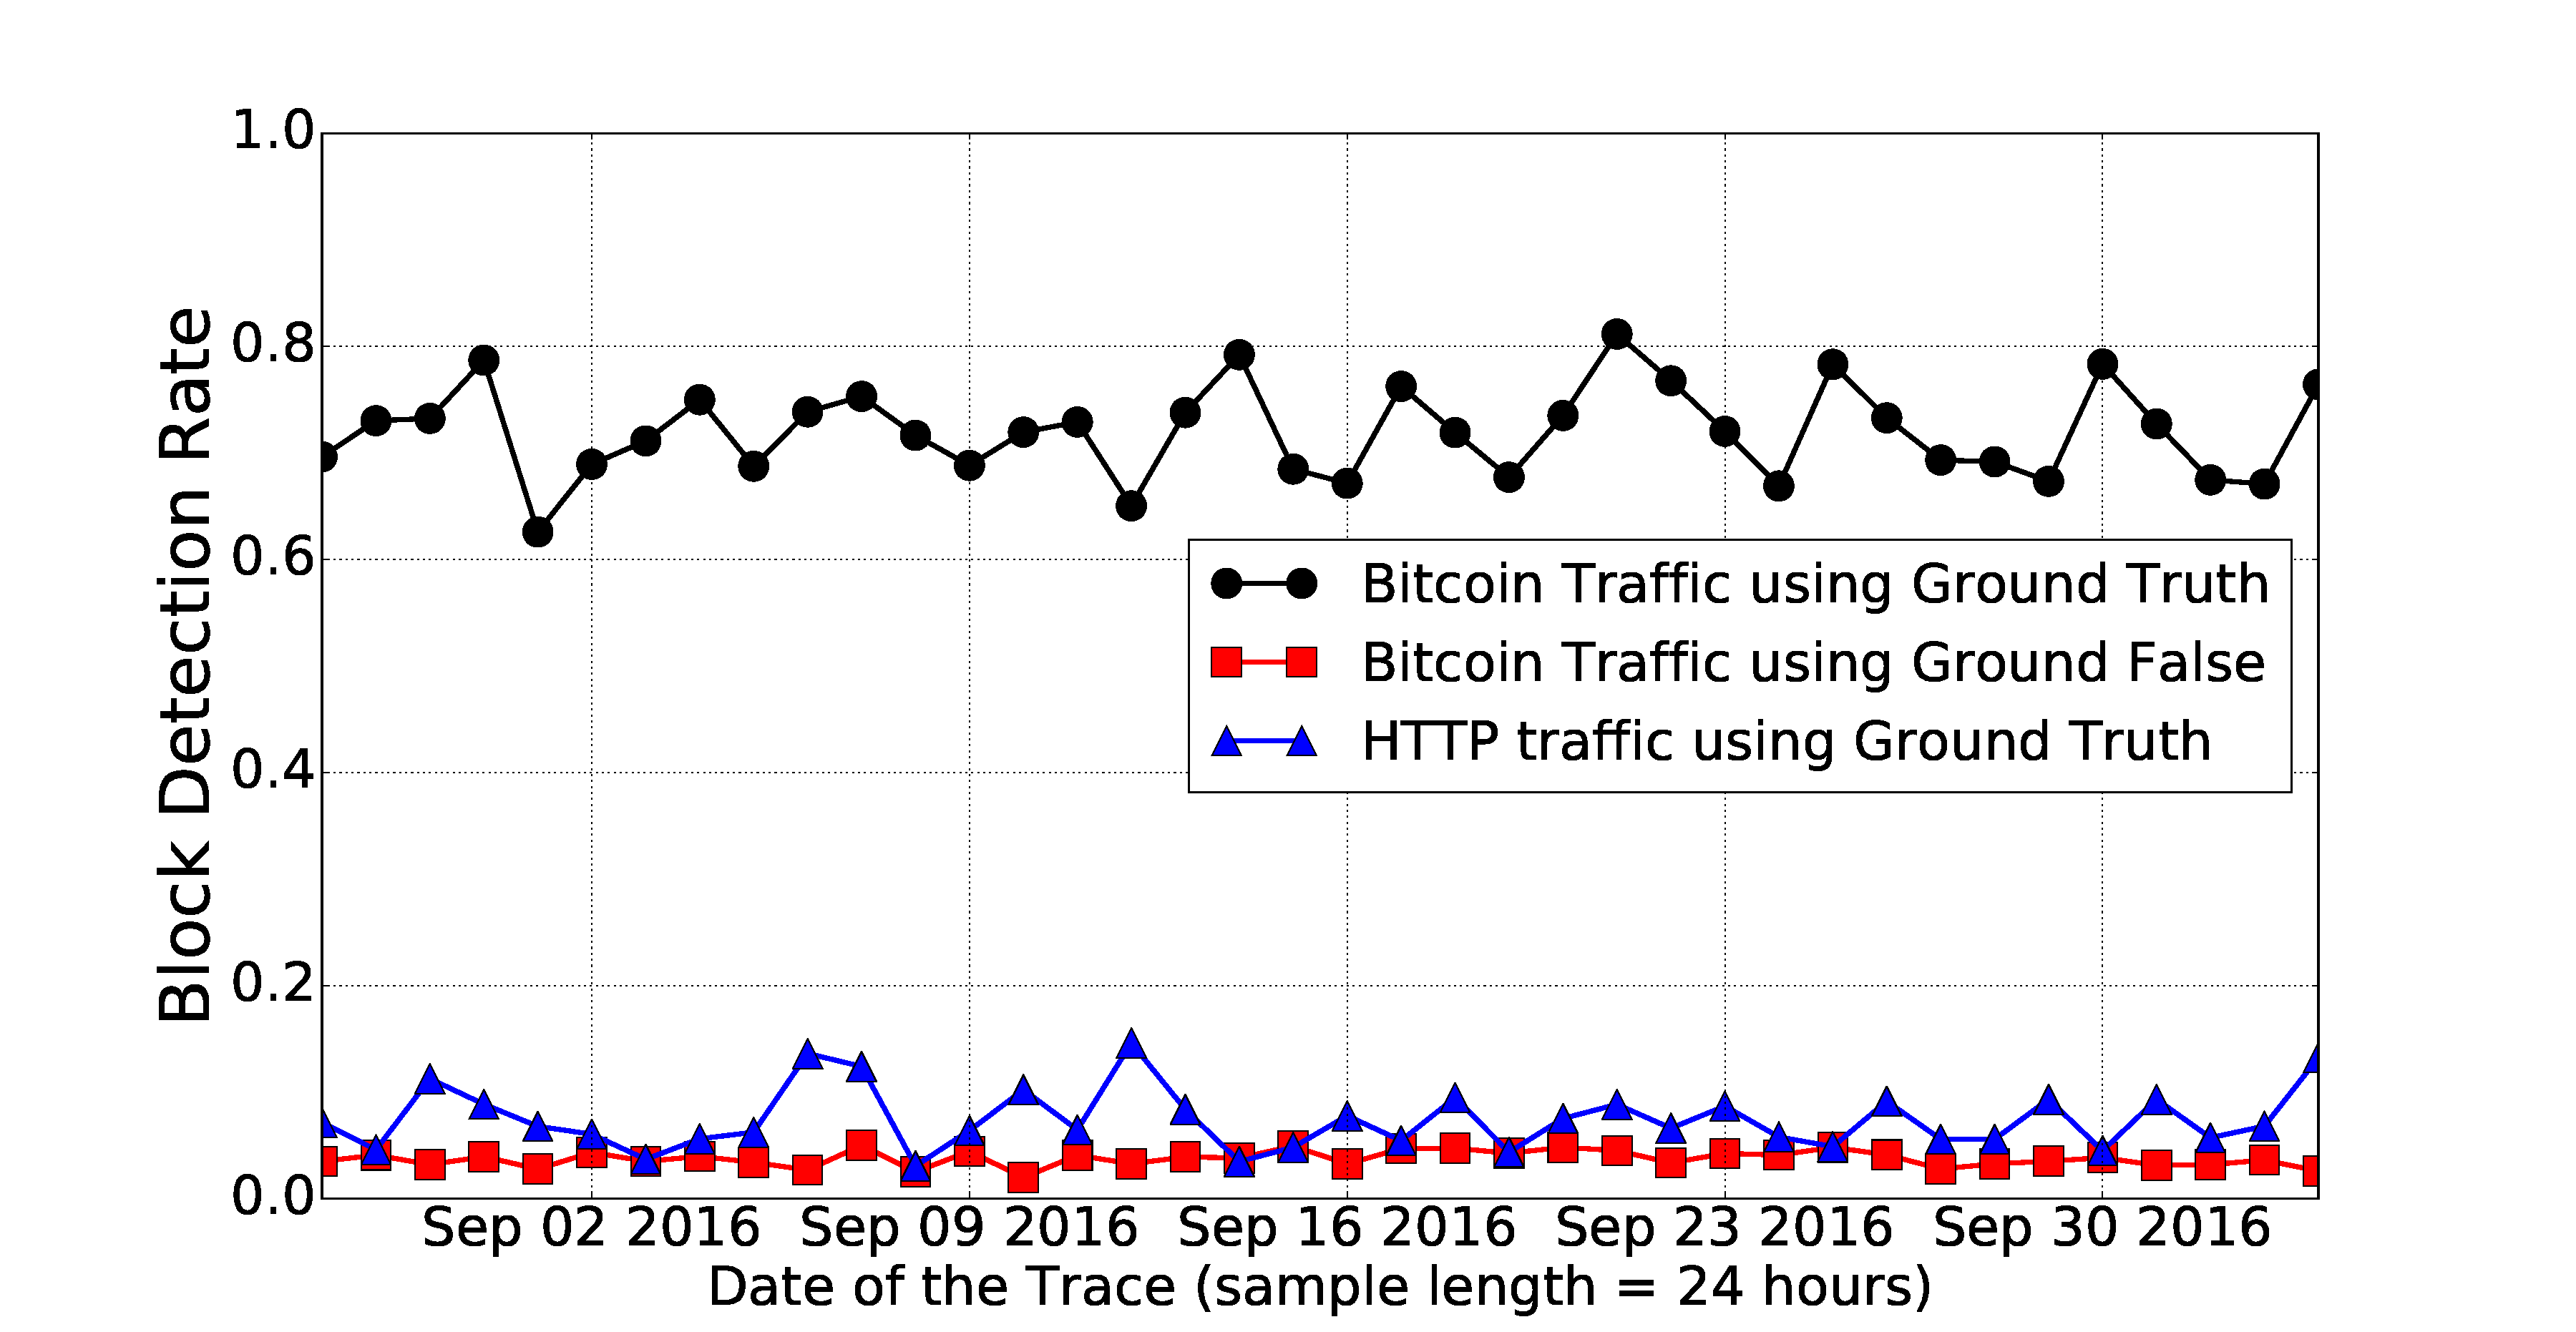
\includegraphics[scale=0.15]{image/jan25/window.pdf}%{image/nov7/window/window.pdf}%roc is also available%window_gf_gt_bitcoin.pdf
\caption{Block detection rate using shape-based classifier}
\label{fig:window}
\end{figure}
\subsection{Neural Network-based Classifier}

We implement the NN-based classifier using Keras~\cite{keras} with Tensorflow~\cite{tensorflow2015-whitepaper} backend. We use complex web and complex CAIDA user to evaluate its performance. Table~\ref{tab:nn} shows the result of NN-based classifier for different sizes of training data. As the table indicates, the accuracy of the classifier improves from $62\%$ to $96\%$ when we increase the size of training data from $1000$ to $40,000$. Note that, true and false positive improves from $44\%$ to $92\%$ and $20\%$ to $2\%$ respectively when we increase the size of training data.
\begin{comment}
To run this classifier, we need to set two parameters: learning rate and epochs.
 Learning rate is a hyper-parameter which controls how much we adjust the weights of the neural network model in each iteration. Moreover, epochs depict the number of times that the algorithm is run on the training data. We use the default value of $0.01$ for the learning rate of Adam optimizer ($lr$). For the epochs, we run our model for values ranging from $50$ to $2000$ and realize that using $1000$ number of epochs we can get a good performance from our classifier. Having a small value for epoch keeps the model from learning the dataset. On the other hand, having a very large number for it may cause over-fitting. Therefore, we need to pick this value very carefully. 
 
 
  Furthermore, increasing the number of epochs would increase the training time. For example, the training time increases from $20$ seconds to around $4$ minutes when we increase the number of epochs from $50$ to $1000$ for $5000$ number of training data. Therefore, we need to take this into account when the size of training data increases.
  \end{comment}
\begin{comment}
\begin{figure}
\centering
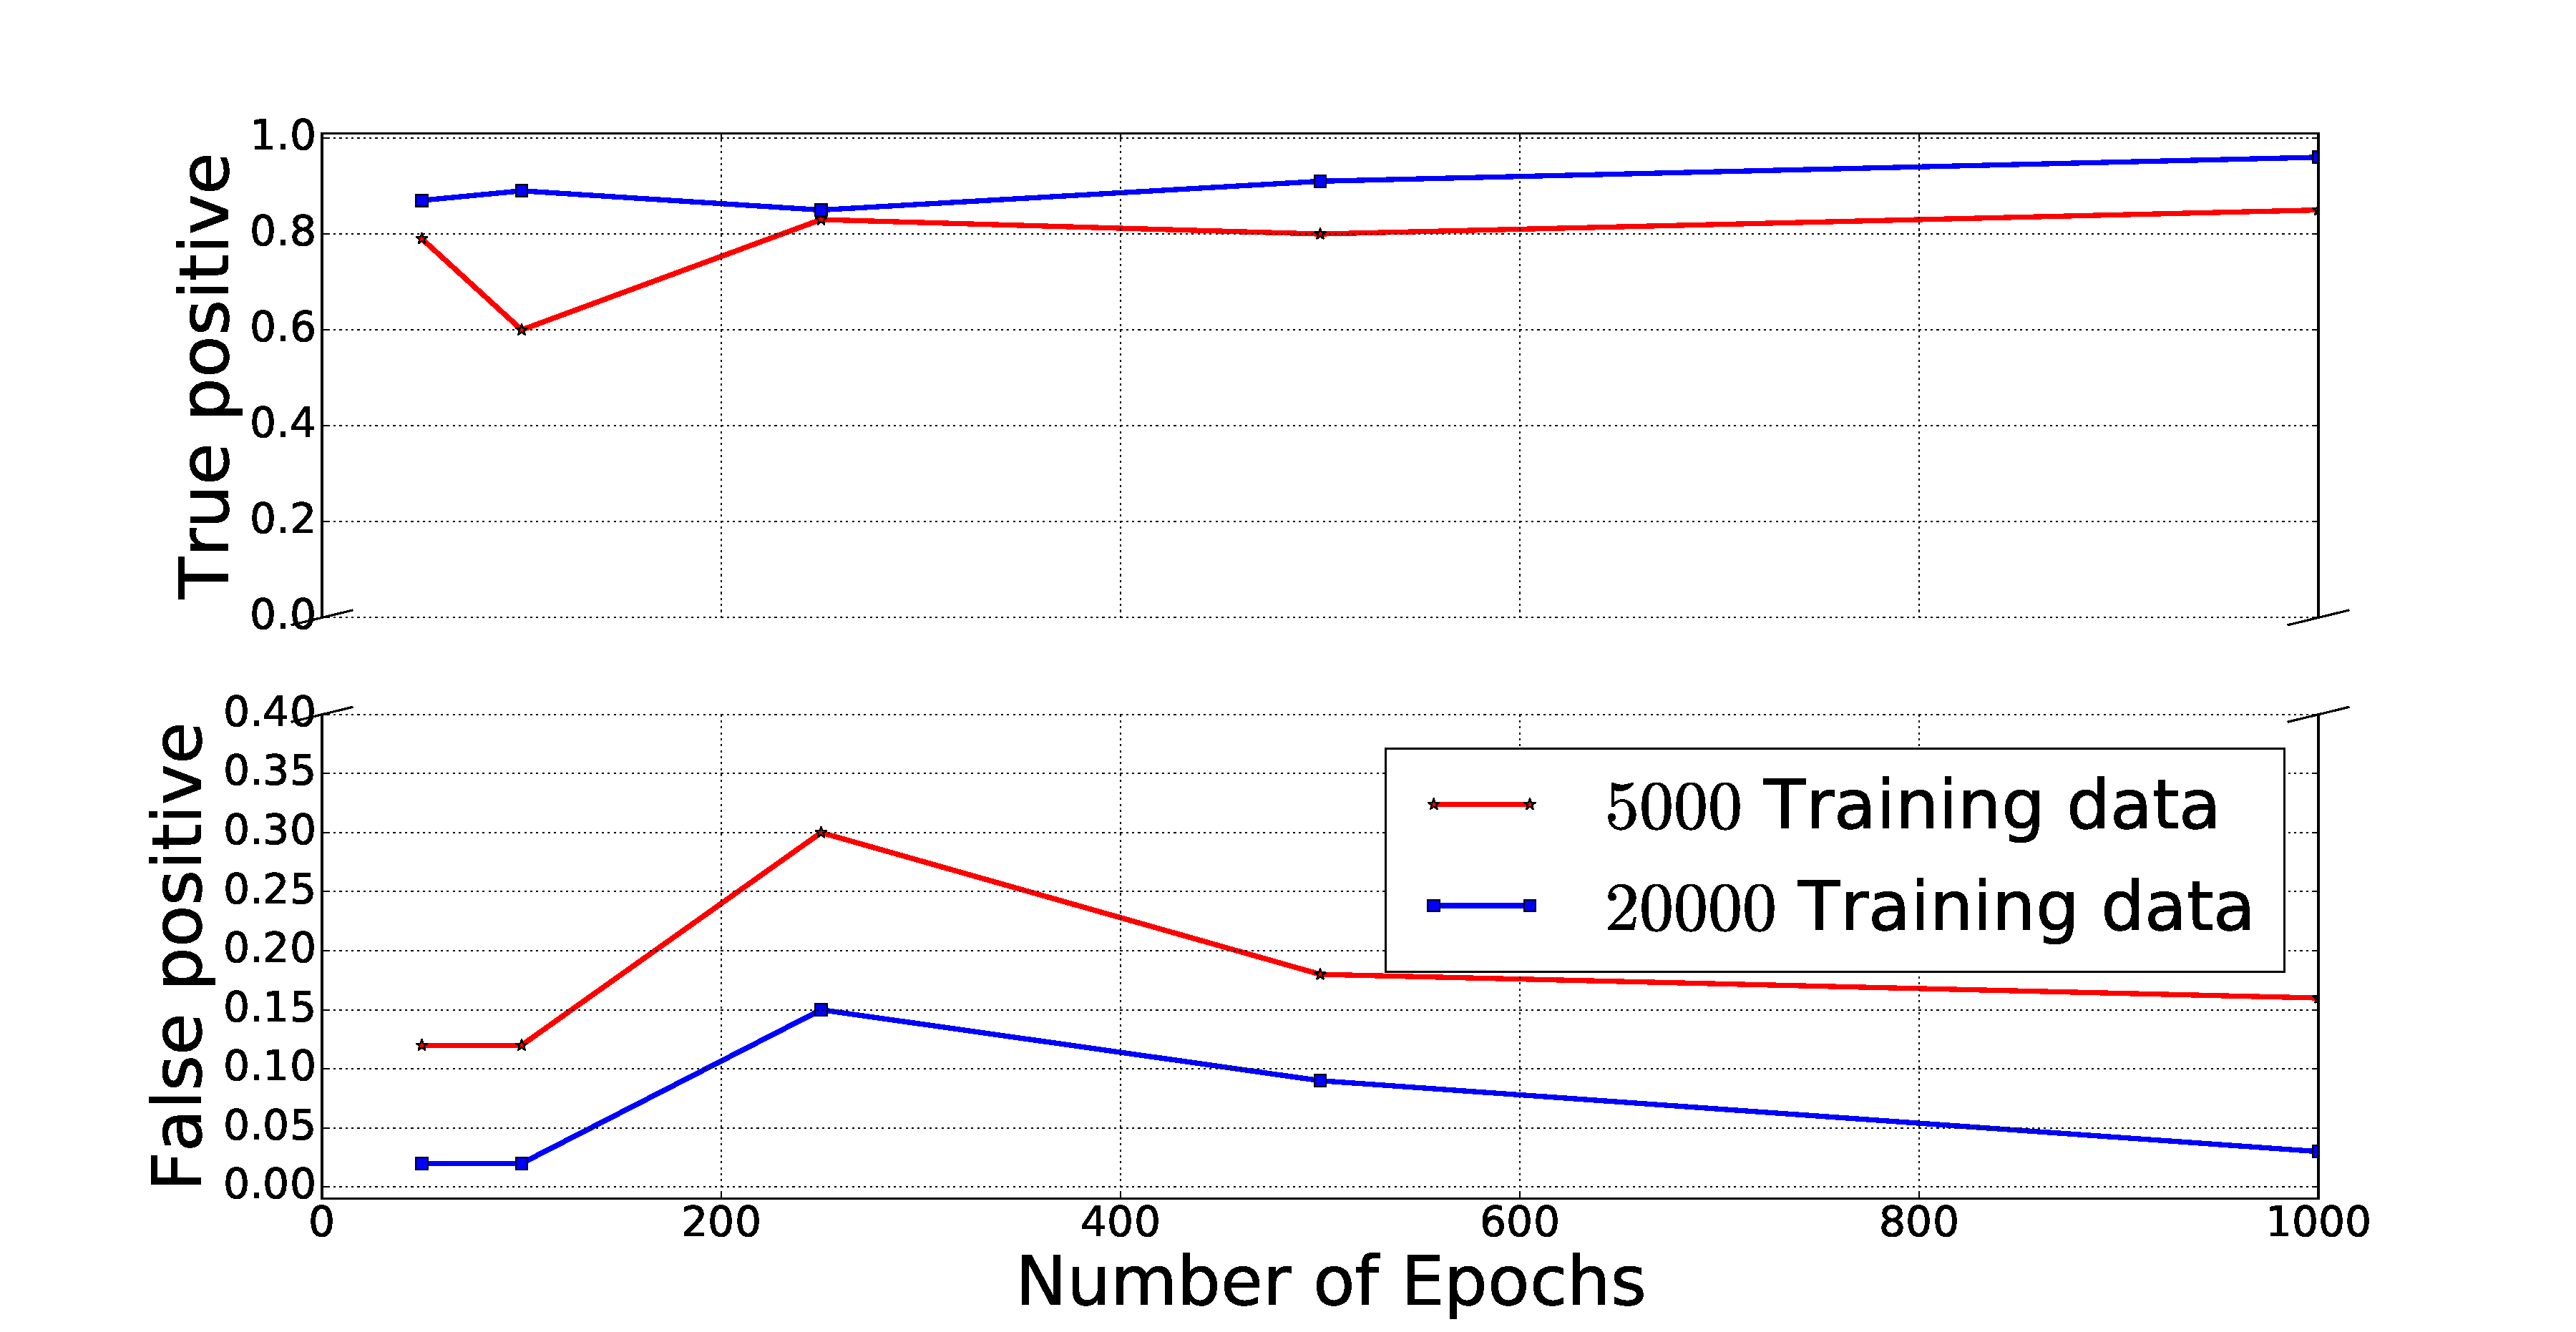
\includegraphics[width=\linewidth]{image/jan25/epochs.pdf}
\caption{Impact of Increasing the number of epochs in performance of the Neural Network Classifier}
\label{fig:epoch}
\end{figure}
\end{comment}

\begin{comment}
\begin{table}[h!]
  \begin{center}
     \caption{Result of Neural Network classifier}
    \label{tab:nn}
    \begin{tabular}{c|c|c|c}
    \kern 0.5pc \shortstack{ Training \\Size}& \shortstack{False Positive\\ ($\%$)} &\shortstack{True Positive\\ ($\%$)}&\shortstack{Accuracy \\($\%$)} \kern 0.5pc\\
      \hline
	$1000$&$20$ &$44 $  & $62$\\
	$5000$&$11$& $80$  & $85$\\
	$10,000$&$6$& $84$  &$ 89$\\
	$80,000$&$0.1$& $93$   & $96$\\% for 1000 epochs
    \end{tabular}
  \end{center}
\end{table}
\end{comment}

\begin{table}
\center \caption{Result of neural network classifier.}\label{tab:nn}
\begin{tabular}{|c|c|c|c|}
\hline
 Training size& False positive ($\%$) &True positive ($\%$)&Accuracy ($\%$)\\
      \hline
	$1000$&$20$ &$44 $  & $62$\\
	$5000$&$11$& $80$  & $85$\\
	$10,000$&$6$& $84$  &$ 89$\\
	$40,000$&$2$& $92$   & $95$\\% for 1000 epochs

	%$80,000$&$0.1$& $93$   & $96$\\% for 1000 epochs
\hline
\end{tabular}
\end{table}



\subsection{Combined Classifier}
To extend the neural network-based classifier, we defined combined classifier, which uses all of the attributes used in previous classifiers. Using this classifier, we reach $99.84\%$ accuracy with false positive of $0$ and true positive of $99.74\%$ having $40,000$ of training data and sample size of $10$ minutes. This result is very promising and shows that having enough data and using the attributes that distinguishes \bc from other traffic, we are able to train a neural network model that gives us $0\%$ false positive and more than $99\%$ accuracy.


\begin{comment}
\begin{table}
\center \caption{Result of combined classifier.}\label{tab:comb}
\begin{tabular}{|c|c|c|c|}
\hline
 Training size& False positive ($\%$) &True positive ($\%$)&Accuracy ($\%$)\\
      \hline
	$5000$    &$0.28$   & $99.73$   & $99.72$\\% for 70 epochs
	$10,000$  &$0.05$   & $99.73$   & $99.84$\\% for 40 epochs
	$20,000$  &$0.085$  & $99.76$   & $99.84$\\% for 10 epochs
	$40,000$  &$0.0$    & $99.74$   & $99.84$\\% for 30 epochs
%$40,000$  &$5e-5$    & $99.64$   & $99.82$\\% for 20 epochs
\hline
\end{tabular}
\end{table}
\end{comment}
\subsection{Summary and Comparison of the Results}

The SizeHist and shape-based work only when there is a very small background noise or no noise (think time of $2$ minutes). Therefore, they are not useful when \bc traffic has a large amount of background noise. To distinguish \bc traffic in the presence of larger noises, we employ NN-based and combined classifiers. The benefit of these classifiers is that they do not have the training phase required in NN-based techniques.

On the other hand, the NN-based classifier and combined classifiers result in a better performance in the presence of higher background noise (complex web and complex CAIDA). The combined classifier outperforms the NN-based by using more features during training. This classifier detects \bc traffic using the complex web and complex CAIDA user explained in ~\ref{simpleuser} with $0\%$ false positive and much higher accuracy ($99.84\%$).


 %In the following, we give a summary of results for size-based, shape-based and NN-based classifiers and then, compare their performance.
\begin{comment}
\begin{compactitem}
\item \textbf{Shape-based Classifier:} This classifier, results in $100\%$ true positive and $0\%$ false positive for full block mode when there is no background noise, but it fails to detect \bc traffic on compact block mode because of the small block sizes. The performance of this classifier quickly diminishes in the presence of small noise such as simple noisy user model described in section~\ref{simpleuser}.
\item \textbf{Size-based Classifiers:} 
In this category, we have SizeHist.% and D2U classifiers.
\begin{itemize}
\item[$\square$] \textbf{SizeHist Classifier:}
Using $10$ minutes of traffic with a think time of $1$ minute, we can reach $0\%$ false positive and more than $90\%$ true positive in both compact and full block modes. Note that it gets a similar result for both cases when we have more than $20$ minutes of 
traffic with a think time of $30$ seconds. 
\end{itemize}
\end{comment}

\begin{comment}
\item[$\square$] \textbf{D2U Classifier:}
This classifier reaches around $80\%$ true positive and up to $5\%$ false positive for both compact and full modes when there are at least $10$ minutes of traffic and the think time is $2$ minutes. 
\end{comment}
\iffalse
\item[$\square$] \textbf{SizeTor Classifier:}
We use this method when the traffic is tunneled over Tor (three pluggable transports and normal Tor).
We reach perfect more than $90\%$ true positive and $0\%$ false positive when we have one tab 
open with zero think time. We increase the noise to see when the results start dropping. 
We learn that increasing the background noise to more than one open tab hugely impacts 
the performance: with two open tabs and $10$ minutes of traffic, we have $40\%$ true positive.
\end{itemize}
\fi
\begin{comment}
The previous classifiers including SizeHist and shape-based work only when there is a very small background noise or no noise (think time of $2$ minutes). Therefore, they are not useful when \bc traffic has a large amount of background noise. To distinguish \bc traffic in the presence of larger noises, we employ NN-based and combined classifiers. The benefit of these classifiers is that they do not have the training phase required in NN-based techniques.
\item \textbf{NN-based Classifier and Combined Classifier:}
To evaluate these classifiers, we use complex web and complex CAIDA users in compact and full block modes. Our NN-based classifier is able to reach near perfect accuracy ($95\%$) with $92\%$ true positive and less than $2\%$ false positive when we the size of training data is $40,000$. More over, using combined classifier which extends the NN-basedclassifier by using more features and largening the model, we can reach more than $99\%$ accuracy with $0$ false positive and more than $99\%$ true positive. Note that the combined classifier outperforms all the previous ones since it is able to detect \bc traffic using complex web and complex CAIDA user explained in ~\ref{simpleuser} with $0\%$ false positive and much higher accuracy ($99.84\%$).
\end{compactitem}
\end{comment}
